This section provides some information on various
implementation details for the RVM runtime system.

\subsection{Object Layout} \label{sssec:objects}
Values in Java\trademark are either {\em primitive} (e.g. {\tt int},
{\tt double}, etc.)  or they are {\em references} (that is, pointers) to
objects.  Objects are either {\em arrays} having components or {\em
simple objects} having fields.  RVM's object model is governed by four
criteria: 
\begin{itemize}
\item{}
field and array accesses should be as fast as possible,
\item{}
null-pointer checks should be performed by the hardware if possible, 
\item{}
virtual method dispatch should be fast, and 
\item{}
other (less frequent) Java\trademark operations  should not be prohibitively slow.
\end{itemize}

Assuming the reference to an object is in a register, the object's
fields can be accessed at a fixed displacement in a single
instruction.  To facilitate array access, the reference to an array
points to the first (zeroth) component of an array and the remaining
components are laid out in ascending order.  The number of components
in an array, its {\em length}, is kept just before its first
component.

\index{NullPointerException}
Java\trademark requires that an attempt to access an object through a {\tt null}
object reference generate a NullPointerException.  In the RVM, references
are machine addresses, and {\tt null} is represented by address $0$.
The AIX operating system permits loads from low memory, but accesses
to very high memory, at small {\em negative} offsets from a null
pointer, normally cause hardware interrupts.\footnote{In AIX, it is at
least theoretically possible for another process to cause a shared
system library to get loaded into very high memory.  This remote
possibility is not a concern in a research project, but would need to
be addressed by a commercial JVM.  It would be sufficient to forbid
read and write access to the last page of addressable memory.
(Accesses to some of the fields of objects bigger than a page could be
checked explicitly without having a major impact on performance.)}
Thus, attempts to index off a null array reference are trapped by
the hardware, because array accesses require loading the array length
which is $-4$ bytes off the array reference.  A hardware null-pointer
check for field accesses is effected by locating fields at negative
offsets from the object reference.

\begin{figure}[htb]
\begin{gif}{object}
\vbox{
\hbox{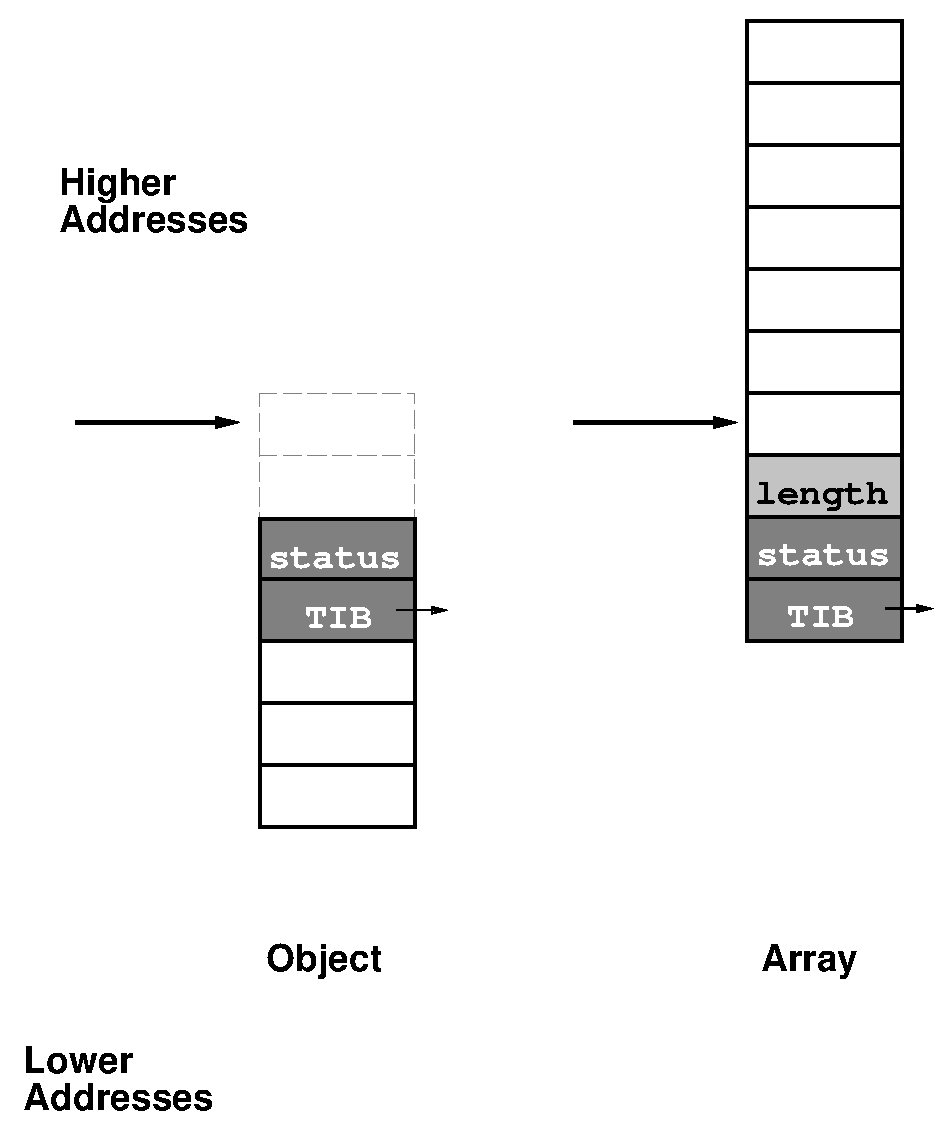
\psfig{file=object.ps,height=3.5in}}
}\hfil
\end{gif}
\caption{Layout of a simple object and an array object in RVM.}
\label{fig:objects}
\end{figure}

\index{field access}
\index{array access}
In summary, in RVM, arrays grow up from the object reference (with the
array length at a fixed negative offset), while simple objects grow
down from the object reference with all fields at a negative offset
(see figure~\ref{fig:objects}).  A field access is accomplished with a
single instruction using base-displacement addressing.  Most array
accesses require three instructions.  A single trap instruction
verifies that the index is within the bounds of the array.  Except for
{\tt byte} (and {\tt boolean}) arrays, the component index must then
be shifted to get a byte index.  The access itself is accomplished
using base-index addressing.

\subsection{Object headers} \label{sssec:headers}
\index{object header}
A two-word object header is associated with each object.  This header
supports virtual method dispatch, dynamic type checking, memory
management, synchronization, and hashing.  It is located $12$ bytes
below the value of a reference to the object.  (This leaves room for
the length field in case the object is an array, see
figure~\ref{fig:objects}.)

\index{locking}
\index{hashing}
One word of the header is a {\em status} word.  The status word is
divided into three {\em bit-fields}.  The first bit-field is used for
locking.  The second bit-field holds
the default hash value of hashed objects.  The third bit-field is used
by the memory management subsystem.  (The size of these bit-fields is
determined by build-time constants.)

\index{TIB}
\index{superclass}
\index{interfaces}
\index{virtual methods}
The other word of an object header is a reference to the {\em Type
Information Block} (TIB) for the object's class. This structure describes
the object's class including its superclass and the interfaces it implements
as well as has pointers to the class' virtual methods.

\subsection{Methods and Fields}\label{sssec:methods}
\index{methods}
\index{JTOC}
\index{TIB}
A compiled method body is an array of machine instructions (stored as
{\tt int}s). 
While the pointers for static fields and methods are stored in the 
{\em Jalapeno Table of Contents} (JTOC),
pointers for instance fields and virtual methods are stored in the class's TIB.
Consequently the dispatch mechanism is different for static and virtual 
methods.

\paragraph{The JTOC}
\index{JTOC}
\begin{figure}[htb]
\begin{gif}{jtoc}
\vbox{
\hbox{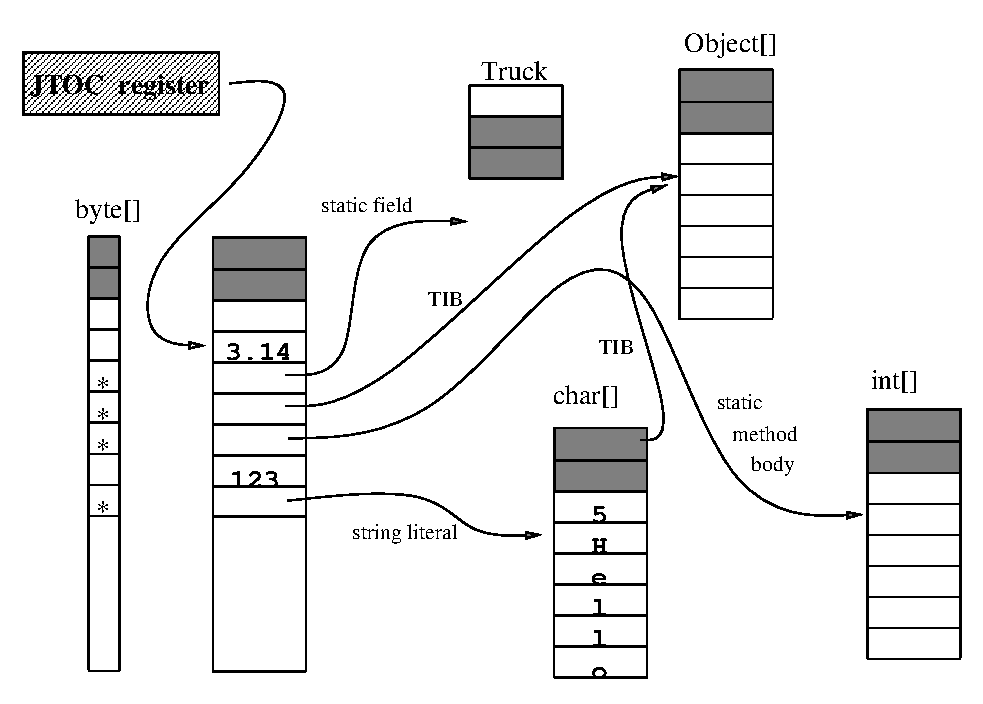
\psfig{file=jtoc.ps,height=3.5in}}
}\hfil
\end{gif}
\caption{The RVM Table Of Contents and other objects.}
\label{fig:jtoc}
\end{figure}
\index{literals}
\index{constants}
\index{dynamic type checking}
All of RVM's global data structures are stored in the JTOC. 
Literals, numeric
constants and references to String constants, are also stored there.
To enable fast common-case dynamic type checking, the JTOC also
contains references to the TIB for each class in the system.  
Since these 
structures can have many types and the JTOC is declared to be an array of 
{\tt int}s  
RVM uses a descriptor array, co-indexed with the JTOC, 
to identify the entries containing references.
A reference to the JTOC is maintained in a dedicated machine register 
(the JTOC register).
The JTOC
is depicted in figure~\ref{fig:jtoc}.  

\paragraph{Virtual Methods}
\index{virtual methods}
A TIB contains pointers to the compiled method 
bodies (executable code) for the virtual methods of its class. 
Thus, the TIB serves as RVM's virtual method table.
A
virtual method dispatch entails loading the TIB pointer at a fixed
offset off the object reference, loading the address of the method
body at a given offset off the TIB pointer, moving this address to the
PowerPC ``link-register'', and executing a branch-and-link --- four
instructions.

\paragraph{Static Fields and Methods} 
\index{static methods}
Static fields and methods are stored in the JTOC. Static method dispatch is 
simpler than virtual dispatch requiring only that the offset of method in the 
JTOC be read to find the address of the method. 

\paragraph{Lazy Method Compilation}
\index{lazy method compilation}
\index{deferred compilation}
\index{lazy method invocation stub}
The slots in the TIB or the JTOC may be filled in with 
a pointer to the compiled code for the method itself or if lazy method 
compilation is enabled and the method has not yet been compiled 
it may be filled in with
a pointer to the compiled code of the {\em lazy method invocation stub}.
If the lazy method invocation stub is invoked its action is to compile the 
method, substitute a pointer to the compiled code of the method in the slot in
the TIB or the JTOC from which it was invoked and then 
cause execution to jump to the start of the compiled method. 

\paragraph{Interface Methods}
\index{interface methods}
\index{IMT}
\index{conflict resolution stub}
Regardless of whether or not a method is overridden in a class that inherits it
virtual method dispatch is still very simple since the method body will be at
the same offset in the TIB in its defining class and in every class that 
inherits from it. 
However, where the method is an interface method, 
that is where it is invoked through an {\tt invoke\_interface} call rather than
an {\tt invoke\_virtual call}, its offset is not the same for every class that 
implements its interface and dispatch is more difficult.
The simplest, and least efficient way, of locating an interface method 
is to search all the virtual method entries in the TIB until a match is found.
Another way uses an {\em Interface Method Table} (IMT) which is much like the 
TIB. Any method that could be an interface method has a fixed offset into the 
IMT just as with the TIB. However, unlike in the TIB, two different methods may
share the same offset into the IMT. In this case, a {\em conflict resolution
stub} is inserted in the IMT. Conflict resolution stubs are
custom-generated machine code sequences that test the value of a
hidden parameter to dispatch to the desired interface method.


\subsection{VM Conventions}
\subsubsection{AIX VM Conventions} \label{aix-conventions}
\index{stack conventions}
\index{register conventions}
\index{calling conventions}

This section describes register, stack, and calling conventions that apply to 
RVM on PowerPC.
Other architectures will require other conventions to maximize performance.

Stackframe layout and calling conventions may evolve as our understanding
of the RVM's performance improves.  Where possible API's should be used
to protect code against such changes.  In particular, we may move to
the AIX conventions at a later date.  Where code differs from the AIX
conventions, it should be marked with a comment to that effect containing
the string "AIX".

\noindent{\bf Register conventions}

Registers (general purpose, gp, and floating point, fp) can be roughly
categorized into four types:

\begin{description}
\item [Scratch]
     Needed for method prologue/epilogue.  Can be used by compiler between
     calls.

\item[Dedicated]
     Reserved registers with known contents:
\begin{description}
\item [JTOC - Jalapeno Table Of Contents]
        Globally accessible data: constants, static fields and methods.

\item [FP - Frame Pointer]
        Current stack frame (thread specific).

\item [TI - Thread (locking) Id]
        Used to set (and test) the locking field of light weight object
        locks.  Can also be shifted to get the index of an object
        representing the current thread in into a global array.

\item [PR - Processor register]
        An object representing the current virtual processor (the one
        executing on the CPU containing these registers).  A field in
        this object contains a reference to the object representing
        the VM\_Thread being executed.
\end{description}

\item [volatile ("caller save", or "parameter")]
     Like scratch registers these can be used by the compiler as 
temporaries,
     but they are not preserved across calls.  (Volatile registers differ
     from scratch registers in that they (the former) can be used to pass
     parameters and result(s) to and from methods.)

\item [Nonvolatile ("callee save", or "preserved")]
     These can be used (and are preserved across calls), but they must be
     saved on method entry and restored at method exit.  Highest numbered
     registers are to be used first.  (At least initially, nonvolatile
     registers will not be used to pass parameters.)

\item[Condition Register's 4-bit fields]
\begin{description}
\item    [CR0 - CR1] scratch

\item    [CR2 - TSCR] dedicated (thread switching, bit 8 TSCRB)

\item    [CR3 - CR7] scratch
\end{description}
\end{description}


\noindent{\bf Stack conventions}

Stacks grow from high memory to low memory.  The stack frame for a method
B called by A is shown in figure~\ref{fig:stackframe}. 
The layout of the stackframe appears in a block comment in
\xlink{{\tt
\$RVM\_ROOT/rvm/src/vm/arch/powerpc/VM\_StackframeLayoutConstants.java}}
{\PPCStackframeLayoutURL}.

\noindent{\bf Calling Conventions}

\begin{description}
\item[Parameters]

    All parameters (that fit) are passed in VOLATILE registers.  Object
    reference and int parameters (or results) consume one GP register; long
    parameters, two gp registers (low-order half in the first);  float and
    double parameters, one fp registers.  Parameters are 
    assigned to registers
    starting with the lowest volatile register through the highest volatile
    register to the highest nonvolatile of the required kind (gp or fp).

    Any additional parameters are passed on the stack in an parameter spill
    area of the caller's stack frame.  The first spilled parameter occupies
    the lowest memory slot.  Slots are filled in the order that parameters
    are spilled.

    An int, or object reference, result is returned in the first volatile
    gp register; a float or double result is returned in the first volatile
    fp register; a long result is returned in the first two volatile gp
    registers (low-order half in the first);

\item [Method prologue responsibilities] (some of these can be omitted for leaf
  methods):

\begin{enumerate}
\item Save the caller's next instruction pointer (callee's return address,
       from the Link Register).

\item Save any nonvolatile floating-point registers used by B.

\item Save any nonvolatile general-purpose registers used by B.

\item Store and update the frame pointer FP.

\item Save B's compiled method ID (eventually, this may not be needed).

\item Check Condition Register bit TSCRB.  If it is set:
         save any of B's parameters that are in volatile registers
         call VM\_Dispatcher.yield();
         restore volatile registers, if necessary
\end{enumerate}

\item [Method epilogue responsibilities]

\begin{enumerate}
\item Restore FP to point to A's stack frame.

\item Restore any nonvolatile general-purpose registers used by B.

\item Restore any nonvolatile floating-point registers used by B.

\item Branch to A's next instruction pointer.
\end{enumerate}
\end{description}

\subsubsection{Lintel VM Conventions} \label{lintel-conventions}
\index{stack conventions}
\index{register conventions}
\index{calling conventions}

This section describes register, stack, and calling conventions that apply to 
RVM on Linux/IA32.

\noindent{\bf Register conventions}

\begin{description}
\item [EAX]
    First GPR parameter register, first GPR result value (high-order part
    of a long result), otherwise volatile (caller-save).

\item[ECX]
    Scratch.

\item[EDX]
    Second GPR parameter register, second GPR result value (low-order part
    of a long result), otherwise volatile (caller-save).

\item[EBX]
    Nonvolatile.

\item[ESP]
    Stack pointer.

\item[EBP]
    Frame pointer, valid at method call/return, must be shadowed in the
    framePointer field of the VM\_Processor object pointed to by ESI (see
    below).

\item[ESI]
    Processor register, reference to the VM\_Processor object for the current
    virtual processor.

\item[EDI]
    Nonvolatile.  (JTOC in baseline compiler)

\end{description}

\noindent{\bf Stack conventions}

Stacks grow from high memory to low memory.  The stack frame for a method
B called by A is shown in figure~\ref{fig:stackframe}. 
The layout of the stackframe appears in a block comment in
\xlink{{\tt
\$RVM\_ROOT/rvm/src/vm/arch/intel/VM\_StackframeLayoutConstants.java}}
{\LintelStackframeLayoutURL}.

\noindent{\bf Calling Conventions}

\begin{description}
\item[At the beginning of B's prologue]
The first two areas of B's stackframe (see above) have been
     established.  ESP points to A's next instruction pointer (2).
     EBP points to A's frame.  If B has (non fp) parameters and
     0 < LINTEL\_PARAMETER\_GPRS, then the first of these is in EAX.
     If B has more than one (non fp) parameters and
     LINTEL\_PARAMETER\_GPRS = 2, then the second of these is in EDX.
     If B has floating-point parameters, then the first
     LINTEL\_PARAMETER\_FPRS of these are at the top of the fp register
     stact (first deepest).
\item[After B's epilogue]
B's stackframe has been removed.  ESP points to the word above where
     B's frame was.  EBP points to A's frame.  (The framePointer field
     of the VM\_Processor object pointed to by ESI must also contain
     this value.)  If B returns a floating-point result, this is at
     the top of the fp register stack.  If B returns a long, the
     low-order word is in EAX and the high-order word is in EDX.
     Otherwise, if B has a result, it is in EAX.

\end{description}

\subsection{Class Loading} \label{sssec:classLoading}
\index{class loading}

RVM implements Java's dynamic class loading. While a class is being loaded it
can be in one of five states. These are
\begin{description}
\item[vacant] a forward reference exists to the class but loading has not yet 
begun.
\item[loaded] the class's bytecode file has been read and parsed successfully.
\item[resolved] the superclass of this class has been loaded and resolved and
the offsets (whether in the object itself, the JTOC, or the class's TIB) of its 
fields and methods have been calculated.
\item[instantiated] the superclass has been instantiated and pointers to the
compiled methods have been inserted into the JTOC(for static methods) and the
TIB (for virtual methods).
\item[initialized] the superclass has been initialized and the class
initializer has been run.
\end{description}

The class passes through these states in the following fashion.

\paragraph{Vacant}
The {\tt VM\_Class} object for this class has been created and registered. 
A class can be in this state if a reference to the class exists in a constant
pool of some other class.

\paragraph{Loaded} 
\index{constant pool}
In this state the class file has been read and parsed.  The constant pool has 
been constructed. The declared methods and fields of the class have been loaded.
Loading a method or field consists of reading its modifiers and attributes.

\paragraph{Resolved}
In this state the superclass of this class has been loaded and resolved. 
A list of the virtual methods and instance fields of this class, including the 
methods and fields
inherited from its superclass has been constructed and the offsets for the 
instance fields have been calculated.  
Space has been allocated in the JTOC for all static fields of the class and for
static method pointers and the appropriate offsets calculated.
The TIB has been initialized and offsets for the virtual methods have been
calculated.

\paragraph{Instantiated}
In this state the superclass of this state has been instantiated. 
The slots in the TIB are filled in with pointers to the compiled code for the 
virtual methods. 
The slots in the JTOC are filled in with pointers to the compiled code for the 
static methods.

\paragraph{Initialized} 
\index{class initializer}
In this state the superclass has been initialized. The class initializer has 
been run. 

\subsection{VM Callbacks}\label{sssec:callbacks}
\index{callbacks}

The RVM provides callbacks for most runtime events of interest to the RVM
programmer, such as classloading, VM bootimage creation, and VM exit.  The
callbacks allow arbitrary code to be executed on any of the supported events.

The callbacks are accessed through the nested interfaces defined in the {\tt
VM\_Callbacks} class.  There is one interface per event type.  To be notified
of an event, register an instance of a class that implements the corresponding
interface with {\tt VM\_Callbacks} by calling the corresponding {\tt add...()}
method.  For example, to be notified when a class is instantiated (see section
\ref{sssec:classLoading}), first implement the {\tt
VM\_Callbacks.ClassInstantiatedMonitor} interface, and then call {\tt
VM\_Callbacks.addClassInstantiatedMonitor()} with an instance of your class.
When any class is instantiated, the {\tt notifyClassInstantiated} method in
your instance will be invoked.

The RVM currently supports callbacks for the following events.
\begin{itemize}
\item {\tt ClassLoaded}, which happens when a class is {\em loaded}.
\item {\tt ClassResolved}, which happens when a class is {\em resolved}.
\item {\tt ClassInstantiated}, which happens when a class is {\em
instantiated}.
\item {\tt ClassInitialized}, which happens when a class is {\em initialized}.
\item {\tt MethodOverride}, which happens when a method in a newly loaded class
overrides a method in an existing class.
\item {\tt ForName}, which happens when java.lang.Class.forName() is invoked.
\item {\tt BootImageWriting}, which happens when boot image writing is started.
\item {\tt Exit}, which happens when the RVM is about to exit.
\end{itemize}
The appropriate interface names can be obtained by appending ``Monitor'' to the
event names (e.g. the interface to implement for the {\tt MethodOverride} event
is {\tt VM\_Callbacks.MethodOverrideMonitor}).  Likewise, the method to
register the callback is ``add'', followed by the name of the interface (e.g.
the register method for the above interface is {\tt
VM\_Callbacks.addMethodOverrideMonitor()}).

NOTE: there is currently no {\tt Startup} event.  It is in the process of being
implemented.

Since the events for which callbacks are available are internal to the RVM,
there are naturally some limitations on the behavior of the callback code.  For
example, as soon as the exit callback is invoked, all threads are considered
daemon threads (i.e. the VM will not wait for any new threads created in the
callbacks to complete before exiting).  Thus, if the exit callback creates any
threads, it has to {\tt join()} with them before returning.  These limitations
may also produce some unexpected behavior.  For example, while there is an
elementary safeguard on any classloading callback that prevents recursive
invocation (i.e. if the callback code itself causes classloading), there is no
such safeguard across events, so, if there are callbacks registered for both
{\tt ClassLoaded} and {\tt ClassInstantiated} events, and the {\tt
ClassInstantiated} callback code causes dynamic class loading, the {\tt
ClassLoaded} callback will be invoked for the new class, but not the {\tt
ClassInstantiated} callback.

Examples of callback use can be seen in the {\tt VM\_Controller} class in the
adaptive system and most {\tt VM\_Allocator} classes.

